%!TEX root = ../rapport.tex
%!TEX encoding = UTF-8 Unicode

% Chapitres "Introduction"

% modifié par Francis Valois, Université Laval
% 31/01/2011 - version 1.0 - Création du document

\chapter{Diagramme physique}
\label{s:physique}

Le diagramme physique est présenté à la figure \ref{fig:diag_physique}. Il est séparé en trois sous-composantes qui sont respectivement : la kinect, la station de base et le robot. Chaque flèche correspond à une interaction entre composantes et peut être soit unidirectionnelle ou bidirectionnelle. De plus, chacun des protocoles ou types d'information sont écrits sur l'interaction pour aider à la compréhension du flux de données dans le projet. Finalement, chacune des boîtes à l'extérieur du rectangle principal correspond à des entrées-sorties nécessaires pour la réussite du projet. Pour permettre une meilleure compréhension du diagramme et éviter une surcharge de celui-ci, les fonctionnalités effectuées par chacune des composantes sont énumérées dans les tableaux \ref{tab:diag_physique1}, \ref{tab:diag_physique2} et \ref{tab:diag_physique3}.


\begin{table}[!ht]
	\caption{Matrice de liaisons entre les composantes physiques et les fonctionnalités effectuées : Kinect} 
	\label{tab:diag_physique1}
	\tabcolsep=0.11cm
	\centering
	\begin{tabular}{|Z{\raggedright}{m}{6.5 cm}|Z{\raggedright}{m}{6.5 cm}|}
	\hline
	Composantes & Fonctionnalités \\ \hline\hline
	\multirow{2}{6.5cm}{Caméra RGB}	& Détecter les obstacles \\ \cline{2-2}
			   						& Localiser le robot \\ \hline
	\multirow{2}{6.5cm}{Caméra infra-rouge} & Détecter les obstacles \\ \cline{2-2}
											& Localiser le robot \\ \hline
	Ordinateur embarqué & Transfert des images de la Kinect vers le Mac mini \\ \hline
	\end{tabular}
\end{table}

\begin{table}[!ht]
	\caption{Matrice de liaisons entre les composantes physiques et les fonctionnalités effectuées : Station de base} 
	\label{tab:diag_physique2}
	\tabcolsep=0.11cm
	\centering
	\begin{tabular}{|Z{\raggedright}{m}{6.5 cm}|Z{\raggedright}{m}{6.5 cm}|}
	\hline
	Composantes & Fonctionnalités \\ \hline\hline
	 & Détecter les obstacles \\ \cline{2-2}
	\multirow{3}{6.5cm}{Ordinateur}& Communiquer entre le robot et la station de base \\ \cline{2-2}
	& Localiser le robot\\ \cline{2-2}
	& Transfert des images de la Kinect vers le Mac mini \\ \hline
	\multirow{7}{6.5cm}{Interface}& Afficher la trajectoire optimale \\ \cline{2-2}
	& Afficher la position du robot\\ \cline{2-2}
	& Afficher le temps d'exécution\\ \cline{2-2}
	& Afficher message d'initiation de la tâche \\ \cline{2-2}
	& Afficher message de fin \\ \cline{2-2}
	& Afficher le cube résolu \\ \hline
	\end{tabular}
\end{table}


\begin{table}[!ht]
	\caption{Matrice de liaisons entre les composantes physiques et les fonctionnalités effectuées : Robot} 
	\label{tab:diag_physique3}
	\tabcolsep=0.11cm
	\centering
	\begin{tabular}{|Z{\raggedright}{m}{6.5 cm}|Z{\raggedright}{m}{8 cm}|}
	\hline
	Composantes & Fonctionnalités \\ \hline\hline
	\multirow{11}{6.5cm}{Mac mini} 	& Détecter les obstacles \\ \cline{2-2}
									& Choisir le cube selon le signal d'antenne \\ \cline{2-2}
									& Calcul de la trajectoire optimale\\ \cline{2-2}
									& Transmettre la trajectoire optimale\\ \cline{2-2}
									& Contrôler le robot pour le dessin \\ \cline{2-2}
									& Commander le préhenseur\\ \cline{2-2}
									& Contrôler la position de la caméra\\ \cline{2-2}
									& Résoudre le cube \\ \cline{2-2}
									& Commander les moteurs \\ \cline{2-2}
									& Allumer la DEL lorsque la tâche est complétée \\ \hline
	Écran LCD & Afficher sur le LCD \\ \hline
	\multirow{6}{6.5cm}{Micro-contrôleur}	& Décodage du signal d'antenne \\ \cline{2-2}
											& Contrôler le robot pour le dessin \\ \cline{2-2}
											& Commander le préhenseur\\ \cline{2-2}
											& Commander les moteurs \\ \cline{2-2}
											& Allumer la DEL lorsque la tâche est complétée \\ \hline
	\multirow{2}{6.5cm}{Batterie} 	& Utiliser une pile rechargeable \\ \cline{2-2}
									& Alimenter les moteurs \\ \hline
	
	Alimentation hacheur 5V & Alimenter les différents périphériques \\ \hline
	Alimentation survolteur 24V & Alimenter l'ordinateur et les différents périphériques\\ \hline
	Pont en H & Commander les moteurs \\ \hline
	Moteurs de déplacement & Se déplacer sans toucher aux obstacles \\ \hline
	Circuit d'antenne & Réception du signal d'antenne \\ \hline
	Antenne & Réception du signal d'antenne \\ \hline
	Moteurs de la caméra & Contrôler la position de la caméra \\ \hline
	Circuit de contrôle des moteur de la caméra & Contrôler la position de la caméra \\ \hline
	Circuit de contrôle de la LED & Allumer la DEL lorsque la tâche est complétée \\ \hline
	Circuit de contrôle du préhenseur & Commander le préhenseur \\ \hline
	\multirow{4}{6.5cm}{Caméra} 	& Détecter les obstacles \\ \cline{2-2}
								& Transmettre les images de la caméra vers le Mac mini \\ \cline{2-2}
								& Lire le cube \\ \hline



	\end{tabular}
\end{table}


\begin{figure}[htbp]
\centering
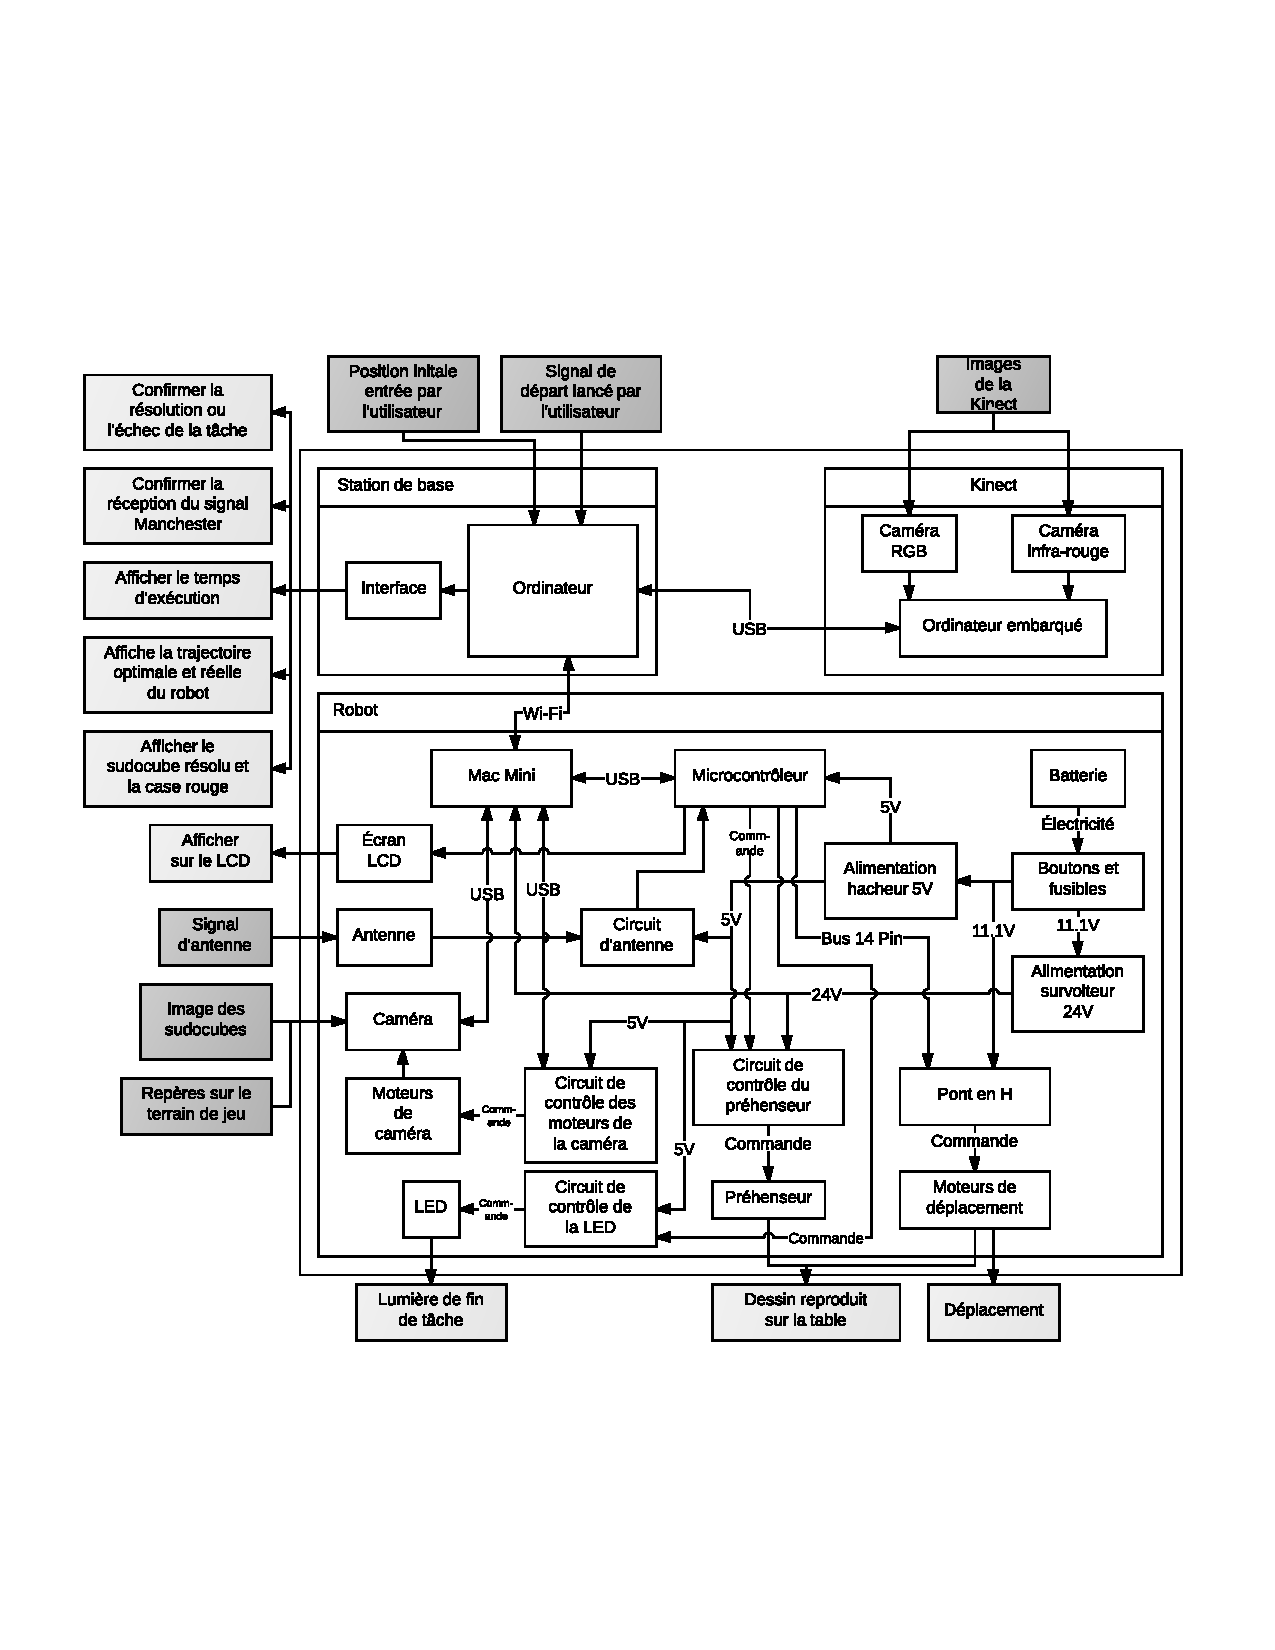
\includegraphics[scale=0.9]{fig/diag_physique.pdf}
\caption{Diagramme physique de l'implantation du robot Kinocto}
\label{fig:diag_physique}
\end{figure}

